%%%%%%%%%%%%%%%%%%%%%%%%%%%%%%%%%%%%%%%%%
% The Legrand Orange Book
% LaTeX Template
% Version 2.1.1 (14/2/16)
%
% This template has been downloaded from:
% http://www.LaTeXTemplates.com
%
% Original author:
% Mathias Legrand (legrand.mathias@gmail.com) with modifications by:
% Vel (vel@latextemplates.com)
%
% License:
% CC BY-NC-SA 3.0 (http://creativecommons.org/licenses/by-nc-sa/3.0/)
%
% Compiling this template:
% This template uses biber for its bibliography and makeindex for its index.
% When you first open the template, compile it from the command line with the 
% commands below to make sure your LaTeX distribution is configured correctly:
%
% 1) pdflatex main
% 2) makeindex main.idx -s StyleInd.ist
% 3) biber main
% 4) pdflatex main x 2
%
% After this, when you wish to update the bibliography/index use the appropriate
% command above and make sure to compile with pdflatex several times 
% afterwards to propagate your changes to the document.
%
% This template also uses a number of packages which may need to be
% updated to the newest versions for the template to compile. It is strongly
% recommended you update your LaTeX distribution if you have any
% compilation errors.
%
% Important note:
% Chapter heading images should have a 2:1 width:height ratio,
% e.g. 920px width and 460px height.
%
%%%%%%%%%%%%%%%%%%%%%%%%%%%%%%%%%%%%%%%%%

%----------------------------------------------------------------------------------------
%	PACKAGES AND OTHER DOCUMENT CONFIGURATIONS
%----------------------------------------------------------------------------------------

\documentclass[11pt,fleqn,a5paper]{book} % Default font size and left-justified equations

%----------------------------------------------------------------------------------------

%%%%%%%%%%%%%%%%%%%%%%%%%%%%%%%%%%%%%%%%%
% The Legrand Orange Book
% Structural Definitions File
% Version 2.0 (9/2/15)
%
% Original author:
% Mathias Legrand (legrand.mathias@gmail.com) with modifications by:
% Vel (vel@latextemplates.com)
% 
% This file has been downloaded from:
% http://www.LaTeXTemplates.com
%
% License:
% CC BY-NC-SA 3.0 (http://creativecommons.org/licenses/by-nc-sa/3.0/)
%
%%%%%%%%%%%%%%%%%%%%%%%%%%%%%%%%%%%%%%%%%

%----------------------------------------------------------------------------------------
%	VARIOUS REQUIRED PACKAGES AND CONFIGURATIONS
%----------------------------------------------------------------------------------------

\usepackage[top=3cm,bottom=3cm,left=3cm,right=3cm,headsep=10pt,a4paper]{geometry} % Page margins

\usepackage{graphicx} % Required for including pictures
\graphicspath{{Pictures/}} % Specifies the directory where pictures are stored

\usepackage{lipsum} % Inserts dummy text

\usepackage{tikz} % Required for drawing custom shapes

\usepackage[english]{babel} % English language/hyphenation

\usepackage{enumitem} % Customize lists
\setlist{nolistsep} % Reduce spacing between bullet points and numbered lists

\usepackage{booktabs} % Required for nicer horizontal rules in tables

\usepackage{xcolor} % Required for specifying colors by name
\definecolor{ocre}{RGB}{243,102,25} % Define the orange color used for highlighting throughout the book

%----------------------------------------------------------------------------------------
%	PERSONAL MODIFICATIONS
%----------------------------------------------------------------------------------------

\usepackage{tipa}
\usepackage{lingmacros}

%----------------------------------------------------------------------------------------
%	FONTS
%----------------------------------------------------------------------------------------

\usepackage{avant} % Use the Avantgarde font for headings
%\usepackage{times} % Use the Times font for headings
\usepackage{mathptmx} % Use the Adobe Times Roman as the default text font together with math symbols from the Sym­bol, Chancery and Com­puter Modern fonts

\usepackage{microtype} % Slightly tweak font spacing for aesthetics
\usepackage[utf8]{inputenc} % Required for including letters with accents
\usepackage[T1]{fontenc} % Use 8-bit encoding that has 256 glyphs

%----------------------------------------------------------------------------------------
%	BIBLIOGRAPHY AND INDEX
%----------------------------------------------------------------------------------------

\usepackage[style=alphabetic,citestyle=numeric,sorting=nyt,sortcites=true,autopunct=true,babel=hyphen,hyperref=true,abbreviate=false,backref=true,backend=biber]{biblatex}
\addbibresource{bibliography.bib} % BibTeX bibliography file
\defbibheading{bibempty}{}

\usepackage{calc} % For simpler calculation - used for spacing the index letter headings correctly
\usepackage{makeidx} % Required to make an index
\makeindex % Tells LaTeX to create the files required for indexing

%----------------------------------------------------------------------------------------
%	MAIN TABLE OF CONTENTS
%----------------------------------------------------------------------------------------

\usepackage{titletoc} % Required for manipulating the table of contents

\contentsmargin{0cm} % Removes the default margin

% Part text styling
\titlecontents{part}[0cm]
{\addvspace{20pt}\centering\large\bfseries}
{}
{}
{}

% Chapter text styling
\titlecontents{chapter}[1.25cm] % Indentation
{\addvspace{12pt}\large\sffamily\bfseries} % Spacing and font options for chapters
{\color{ocre!60}\contentslabel[\Large\thecontentslabel]{1.25cm}\color{ocre}} % Chapter number
{\color{ocre}}  
{\color{ocre!60}\normalsize\;\titlerule*[.5pc]{.}\;\thecontentspage} % Page number

% Section text styling
\titlecontents{section}[1.25cm] % Indentation
{\addvspace{3pt}\sffamily\bfseries} % Spacing and font options for sections
{\contentslabel[\thecontentslabel]{1.25cm}} % Section number
{}
{\hfill\color{black}\thecontentspage} % Page number
[]

% Subsection text styling
\titlecontents{subsection}[1.25cm] % Indentation
{\addvspace{1pt}\sffamily\small} % Spacing and font options for subsections
{\contentslabel[\thecontentslabel]{1.25cm}} % Subsection number
{}
{\ \titlerule*[.5pc]{.}\;\thecontentspage} % Page number
[]

% List of figures
\titlecontents{figure}[0em]
{\addvspace{-5pt}\sffamily}
{\thecontentslabel\hspace*{1em}}
{}
{\ \titlerule*[.5pc]{.}\;\thecontentspage}
[]

% List of tables
\titlecontents{table}[0em]
{\addvspace{-5pt}\sffamily}
{\thecontentslabel\hspace*{1em}}
{}
{\ \titlerule*[.5pc]{.}\;\thecontentspage}
[]

%----------------------------------------------------------------------------------------
%	MINI TABLE OF CONTENTS IN PART HEADS
%----------------------------------------------------------------------------------------

% Chapter text styling
\titlecontents{lchapter}[0em] % Indenting
{\addvspace{15pt}\large\sffamily\bfseries} % Spacing and font options for chapters
{\color{ocre}\contentslabel[\Large\thecontentslabel]{1.25cm}\color{ocre}} % Chapter number
{}  
{\color{ocre}\normalsize\sffamily\bfseries\;\titlerule*[.5pc]{.}\;\thecontentspage} % Page number

% Section text styling
\titlecontents{lsection}[0em] % Indenting
{\sffamily\small} % Spacing and font options for sections
{\contentslabel[\thecontentslabel]{1.25cm}} % Section number
{}
{}

% Subsection text styling
\titlecontents{lsubsection}[.5em] % Indentation
{\normalfont\footnotesize\sffamily} % Font settings
{}
{}
{}

%----------------------------------------------------------------------------------------
%	PAGE HEADERS
%----------------------------------------------------------------------------------------

\usepackage{fancyhdr} % Required for header and footer configuration

\pagestyle{fancy}
\renewcommand{\chaptermark}[1]{\markboth{\sffamily\normalsize\bfseries\chaptername\ \thechapter.\ #1}{}} % Chapter text font settings
\renewcommand{\sectionmark}[1]{\markright{\sffamily\normalsize\thesection\hspace{5pt}#1}{}} % Section text font settings
\fancyhf{} \fancyhead[LE,RO]{\sffamily\normalsize\thepage} % Font setting for the page number in the header
\fancyhead[LO]{\rightmark} % Print the nearest section name on the left side of odd pages
\fancyhead[RE]{\leftmark} % Print the current chapter name on the right side of even pages
\renewcommand{\headrulewidth}{0.5pt} % Width of the rule under the header
\addtolength{\headheight}{2.5pt} % Increase the spacing around the header slightly
\renewcommand{\footrulewidth}{0pt} % Removes the rule in the footer
\fancypagestyle{plain}{\fancyhead{}\renewcommand{\headrulewidth}{0pt}} % Style for when a plain pagestyle is specified

% Removes the header from odd empty pages at the end of chapters
\makeatletter
\renewcommand{\cleardoublepage}{
\clearpage\ifodd\c@page\else
\hbox{}
\vspace*{\fill}
\thispagestyle{empty}
\newpage
\fi}

%----------------------------------------------------------------------------------------
%	THEOREM STYLES
%----------------------------------------------------------------------------------------

\usepackage{amsmath,amsfonts,amssymb,amsthm} % For math equations, theorems, symbols, etc

\newcommand{\intoo}[2]{\mathopen{]}#1\,;#2\mathclose{[}}
\newcommand{\ud}{\mathop{\mathrm{{}d}}\mathopen{}}
\newcommand{\intff}[2]{\mathopen{[}#1\,;#2\mathclose{]}}
\newtheorem{notation}{Notation}[chapter]

% Boxed/framed environments
\newtheoremstyle{ocrenumbox}% % Theorem style name
{0pt}% Space above
{0pt}% Space below
{\normalfont}% % Body font
{}% Indent amount
{\small\bf\sffamily\color{ocre}}% % Theorem head font
{\;}% Punctuation after theorem head
{0.25em}% Space after theorem head
{\small\sffamily\color{ocre}\thmname{#1}\nobreakspace\thmnumber{\@ifnotempty{#1}{}\@upn{#2}}% Theorem text (e.g. Theorem 2.1)
\thmnote{\nobreakspace\the\thm@notefont\sffamily\bfseries\color{black}---\nobreakspace#3.}} % Optional theorem note
\renewcommand{\qedsymbol}{$\blacksquare$}% Optional qed square

\newtheoremstyle{blacknumex}% Theorem style name
{5pt}% Space above
{5pt}% Space below
{\normalfont}% Body font
{} % Indent amount
{\small\bf\sffamily}% Theorem head font
{\;}% Punctuation after theorem head
{0.25em}% Space after theorem head
{\small\sffamily{\tiny\ensuremath{\blacksquare}}\nobreakspace\thmname{#1}\nobreakspace\thmnumber{\@ifnotempty{#1}{}\@upn{#2}}% Theorem text (e.g. Theorem 2.1)
\thmnote{\nobreakspace\the\thm@notefont\sffamily\bfseries---\nobreakspace#3.}}% Optional theorem note

\newtheoremstyle{blacknumbox} % Theorem style name
{0pt}% Space above
{0pt}% Space below
{\normalfont}% Body font
{}% Indent amount
{\small\bf\sffamily}% Theorem head font
{\;}% Punctuation after theorem head
{0.25em}% Space after theorem head
{\small\sffamily\thmname{#1}\nobreakspace\thmnumber{\@ifnotempty{#1}{}\@upn{#2}}% Theorem text (e.g. Theorem 2.1)
\thmnote{\nobreakspace\the\thm@notefont\sffamily\bfseries---\nobreakspace#3.}}% Optional theorem note

% Non-boxed/non-framed environments
\newtheoremstyle{ocrenum}% % Theorem style name
{5pt}% Space above
{5pt}% Space below
{\normalfont}% % Body font
{}% Indent amount
{\small\bf\sffamily\color{ocre}}% % Theorem head font
{\;}% Punctuation after theorem head
{0.25em}% Space after theorem head
{\small\sffamily\color{ocre}\thmname{#1}\nobreakspace\thmnumber{\@ifnotempty{#1}{}\@upn{#2}}% Theorem text (e.g. Theorem 2.1)
\thmnote{\nobreakspace\the\thm@notefont\sffamily\bfseries\color{black}---\nobreakspace#3.}} % Optional theorem note
\renewcommand{\qedsymbol}{$\blacksquare$}% Optional qed square
\makeatother

% Defines the theorem text style for each type of theorem to one of the three styles above
\newcounter{dummy} 
\numberwithin{dummy}{section}
\theoremstyle{ocrenumbox}
\newtheorem{theoremeT}[dummy]{Theorem}
\newtheorem{problem}{Problem}[chapter]
\newtheorem{exerciseT}{Exercise}[chapter]
\theoremstyle{blacknumex}
\newtheorem{exampleT}{Example}[chapter]
\theoremstyle{blacknumbox}
\newtheorem{vocabulary}{Vocabulary}[chapter]
\newtheorem{definitionT}{Definition}[section]
\newtheorem{corollaryT}[dummy]{Corollary}
\theoremstyle{ocrenum}
\newtheorem{proposition}[dummy]{Proposition}

%----------------------------------------------------------------------------------------
%	DEFINITION OF COLORED BOXES
%----------------------------------------------------------------------------------------

\RequirePackage[framemethod=default]{mdframed} % Required for creating the theorem, definition, exercise and corollary boxes

% Theorem box
\newmdenv[skipabove=7pt,
skipbelow=7pt,
backgroundcolor=black!5,
linecolor=ocre,
innerleftmargin=5pt,
innerrightmargin=5pt,
innertopmargin=5pt,
leftmargin=0cm,
rightmargin=0cm,
innerbottommargin=5pt]{tBox}

% Exercise box	  
\newmdenv[skipabove=7pt,
skipbelow=7pt,
rightline=false,
leftline=true,
topline=false,
bottomline=false,
backgroundcolor=ocre!10,
linecolor=ocre,
innerleftmargin=5pt,
innerrightmargin=5pt,
innertopmargin=5pt,
innerbottommargin=5pt,
leftmargin=0cm,
rightmargin=0cm,
linewidth=4pt]{eBox}	

% Definition box
\newmdenv[skipabove=7pt,
skipbelow=7pt,
rightline=false,
leftline=true,
topline=false,
bottomline=false,
linecolor=ocre,
innerleftmargin=5pt,
innerrightmargin=5pt,
innertopmargin=0pt,
leftmargin=0cm,
rightmargin=0cm,
linewidth=4pt,
innerbottommargin=0pt]{dBox}	

% Corollary box
\newmdenv[skipabove=7pt,
skipbelow=7pt,
rightline=false,
leftline=true,
topline=false,
bottomline=false,
linecolor=gray,
backgroundcolor=black!5,
innerleftmargin=5pt,
innerrightmargin=5pt,
innertopmargin=5pt,
leftmargin=0cm,
rightmargin=0cm,
linewidth=4pt,
innerbottommargin=5pt]{cBox}

\newmdenv[skipabove=7pt,
skipbelow=7pt,
rightline=false,
leftline=true,
topline=false,
bottomline=false,
linecolor=gray,
backgroundcolor=black!5,
innerleftmargin=15pt,
innerrightmargin=5pt,
innertopmargin=5pt,
leftmargin=0cm,
rightmargin=0cm,
linewidth=4pt,
innerbottommargin=5pt]{sBox}

% Creates an environment for each type of theorem and assigns it a theorem text style from the "Theorem Styles" section above and a colored box from above
\newenvironment{theorem}{\begin{tBox}\begin{theoremeT}}{\end{theoremeT}\end{tBox}}
\newenvironment{exercise}{\begin{eBox}\begin{exerciseT}}{\hfill{\color{ocre}\tiny\ensuremath{\blacksquare}}\end{exerciseT}\end{eBox}}				  
\newenvironment{definition}{\begin{dBox}\begin{definitionT}}{\end{definitionT}\end{dBox}}	
\newenvironment{example}{\begin{exampleT}}{\hfill{\tiny\ensuremath{\blacksquare}}\end{exampleT}}		
\newenvironment{corollary}{\begin{cBox}\begin{corollaryT}}{\end{corollaryT}\end{cBox}}
\newenvironment{sentence}{\begin{sBox}}{\end{sBox}}

%----------------------------------------------------------------------------------------
%	REMARK ENVIRONMENT
%----------------------------------------------------------------------------------------

\newenvironment{remark}{\par\vspace{10pt}\small % Vertical white space above the remark and smaller font size
\begin{list}{}{
\leftmargin=35pt % Indentation on the left
\rightmargin=25pt}\item\ignorespaces % Indentation on the right
\makebox[-2.5pt]{\begin{tikzpicture}[overlay]
\node[draw=ocre!60,line width=1pt,circle,fill=ocre!25,font=\sffamily\bfseries,inner sep=2pt,outer sep=0pt] at (-15pt,0pt){\textcolor{ocre}{R}};\end{tikzpicture}} % Orange R in a circle
\advance\baselineskip -1pt}{\end{list}\vskip5pt} % Tighter line spacing and white space after remark

%----------------------------------------------------------------------------------------
%	SECTION NUMBERING IN THE MARGIN
%----------------------------------------------------------------------------------------

\makeatletter
\renewcommand{\@seccntformat}[1]{\llap{\textcolor{ocre}{\csname the#1\endcsname}\hspace{1em}}}                    
\renewcommand{\section}{\@startsection{section}{1}{\z@}
{-4ex \@plus -1ex \@minus -.4ex}
{1ex \@plus.2ex }
{\normalfont\large\sffamily\bfseries}}
\renewcommand{\subsection}{\@startsection {subsection}{2}{\z@}
{-3ex \@plus -0.1ex \@minus -.4ex}
{0.5ex \@plus.2ex }
{\normalfont\sffamily\bfseries}}
\renewcommand{\subsubsection}{\@startsection {subsubsection}{3}{\z@}
{-2ex \@plus -0.1ex \@minus -.2ex}
{.2ex \@plus.2ex }
{\normalfont\small\sffamily\bfseries}}                        
\renewcommand\paragraph{\@startsection{paragraph}{4}{\z@}
{-2ex \@plus-.2ex \@minus .2ex}
{.1ex}
{\normalfont\small\sffamily\bfseries}}

%----------------------------------------------------------------------------------------
%	PART HEADINGS
%----------------------------------------------------------------------------------------

% numbered part in the table of contents
\newcommand{\@mypartnumtocformat}[2]{%
\setlength\fboxsep{0pt}%
\noindent\colorbox{ocre!20}{\strut\parbox[c][.7cm]{\ecart}{\color{ocre!70}\Large\sffamily\bfseries\centering#1}}\hskip\esp\colorbox{ocre!40}{\strut\parbox[c][.7cm]{\linewidth-\ecart-\esp}{\Large\sffamily\centering#2}}}%
%%%%%%%%%%%%%%%%%%%%%%%%%%%%%%%%%%
% unnumbered part in the table of contents
\newcommand{\@myparttocformat}[1]{%
\setlength\fboxsep{0pt}%
\noindent\colorbox{ocre!40}{\strut\parbox[c][.7cm]{\linewidth}{\Large\sffamily\centering#1}}}%
%%%%%%%%%%%%%%%%%%%%%%%%%%%%%%%%%%
\newlength\esp
\setlength\esp{4pt}
\newlength\ecart
\setlength\ecart{1.2cm-\esp}
\newcommand{\thepartimage}{}%
\newcommand{\partimage}[1]{\renewcommand{\thepartimage}{#1}}%
\def\@part[#1]#2{%
\ifnum \c@secnumdepth >-2\relax%
\refstepcounter{part}%
\addcontentsline{toc}{part}{\texorpdfstring{\protect\@mypartnumtocformat{\thepart}{#1}}{\partname~\thepart\ ---\ #1}}
\else%
\addcontentsline{toc}{part}{\texorpdfstring{\protect\@myparttocformat{#1}}{#1}}%
\fi%
\startcontents%
\markboth{}{}%
{\thispagestyle{empty}%
\begin{tikzpicture}[remember picture,overlay]%
\node at (current page.north west){\begin{tikzpicture}[remember picture,overlay]%	
\fill[ocre!20](0cm,0cm) rectangle (\paperwidth,-\paperheight);
\node[anchor=north] at (4cm,-3.25cm){\color{ocre!40}\fontsize{220}{100}\sffamily\bfseries\@Roman\c@part}; 
\node[anchor=south east] at (\paperwidth-1cm,-\paperheight+1cm){\parbox[t][][t]{8.5cm}{
\printcontents{l}{0}{\setcounter{tocdepth}{1}}%
}};
\node[anchor=north east] at (\paperwidth-1.5cm,-3.25cm){\parbox[t][][t]{15cm}{\strut\raggedleft\color{white}\fontsize{30}{30}\sffamily\bfseries#2}};
\end{tikzpicture}};
\end{tikzpicture}}%
\@endpart}
\def\@spart#1{%
\startcontents%
\phantomsection
{\thispagestyle{empty}%
\begin{tikzpicture}[remember picture,overlay]%
\node at (current page.north west){\begin{tikzpicture}[remember picture,overlay]%	
\fill[ocre!20](0cm,0cm) rectangle (\paperwidth,-\paperheight);
\node[anchor=north east] at (\paperwidth-1.5cm,-3.25cm){\parbox[t][][t]{15cm}{\strut\raggedleft\color{white}\fontsize{30}{30}\sffamily\bfseries#1}};
\end{tikzpicture}};
\end{tikzpicture}}
\addcontentsline{toc}{part}{\texorpdfstring{%
\setlength\fboxsep{0pt}%
\noindent\protect\colorbox{ocre!40}{\strut\protect\parbox[c][.7cm]{\linewidth}{\Large\sffamily\protect\centering #1\quad\mbox{}}}}{#1}}%
\@endpart}
\def\@endpart{\vfil\newpage
\if@twoside
\if@openright
\null
\thispagestyle{empty}%
\newpage
\fi
\fi
\if@tempswa
\twocolumn
\fi}

%----------------------------------------------------------------------------------------
%	CHAPTER HEADINGS
%----------------------------------------------------------------------------------------

% A switch to conditionally include a picture, implemented by  Christian Hupfer
\newif\ifusechapterimage
\usechapterimagetrue
\newcommand{\thechapterimage}{}%
\newcommand{\chapterimage}[1]{\ifusechapterimage\renewcommand{\thechapterimage}{#1}\fi}%
\def\@makechapterhead#1{%
{\parindent \z@ \raggedright \normalfont
\ifnum \c@secnumdepth >\m@ne
\if@mainmatter
\begin{tikzpicture}[remember picture,overlay]
\node at (current page.north west)
{\begin{tikzpicture}[remember picture,overlay]
\node[anchor=north west,inner sep=0pt] at (0,0) {\ifusechapterimage\includegraphics[width=\paperwidth]{\thechapterimage}\fi};
\draw[anchor=west] (\Gm@lmargin,-9cm) node [line width=2pt,rounded corners=15pt,draw=ocre,fill=white,fill opacity=0.5,inner sep=15pt]{\strut\makebox[22cm]{}};
\draw[anchor=west] (\Gm@lmargin+.3cm,-9cm) node {\huge\sffamily\bfseries\color{black}\thechapter. #1\strut};
\end{tikzpicture}};
\end{tikzpicture}
\else
\begin{tikzpicture}[remember picture,overlay]
\node at (current page.north west)
{\begin{tikzpicture}[remember picture,overlay]
\node[anchor=north west,inner sep=0pt] at (0,0) {\ifusechapterimage\includegraphics[width=\paperwidth]{\thechapterimage}\fi};
\draw[anchor=west] (\Gm@lmargin,-9cm) node [line width=2pt,rounded corners=15pt,draw=ocre,fill=white,fill opacity=0.5,inner sep=15pt]{\strut\makebox[22cm]{}};
\draw[anchor=west] (\Gm@lmargin+.3cm,-9cm) node {\huge\sffamily\bfseries\color{black}#1\strut};
\end{tikzpicture}};
\end{tikzpicture}
\fi\fi\par\vspace*{270\p@}}}

%-------------------------------------------

\def\@makeschapterhead#1{%
\begin{tikzpicture}[remember picture,overlay]
\node at (current page.north west)
{\begin{tikzpicture}[remember picture,overlay]
\node[anchor=north west,inner sep=0pt] at (0,0) {\ifusechapterimage\includegraphics[width=\paperwidth]{\thechapterimage}\fi};
\draw[anchor=west] (\Gm@lmargin,-9cm) node [line width=2pt,rounded corners=15pt,draw=ocre,fill=white,fill opacity=0.5,inner sep=15pt]{\strut\makebox[22cm]{}};
\draw[anchor=west] (\Gm@lmargin+.3cm,-9cm) node {\huge\sffamily\bfseries\color{black}#1\strut};
\end{tikzpicture}};
\end{tikzpicture}
\par\vspace*{270\p@}}
\makeatother

%----------------------------------------------------------------------------------------
%	HYPERLINKS IN THE DOCUMENTS
%----------------------------------------------------------------------------------------

\usepackage{hyperref}
\hypersetup{hidelinks,backref=true,pagebackref=true,hyperindex=true,colorlinks=false,breaklinks=true,urlcolor= ocre,bookmarks=true,bookmarksopen=false,pdftitle={Title},pdfauthor={Author}}
\usepackage{bookmark}
\bookmarksetup{
open,
numbered,
addtohook={%
\ifnum\bookmarkget{level}=0 % chapter
\bookmarksetup{bold}%
\fi
\ifnum\bookmarkget{level}=-1 % part
\bookmarksetup{color=ocre,bold}%
\fi
}
}
 % Insert the commands.tex file which contains the majority of the structure behind the template

\begin{document}

%----------------------------------------------------------------------------------------
%	TITLE PAGE
%----------------------------------------------------------------------------------------

\begingroup
\thispagestyle{empty}
\begin{tikzpicture}[remember picture,overlay]
\coordinate [below=12cm] (midpoint) at (current page.north);
\node at (current page.north west)
{\begin{tikzpicture}[remember picture,overlay]
\node[anchor=north west,inner sep=0pt] at (0,0) {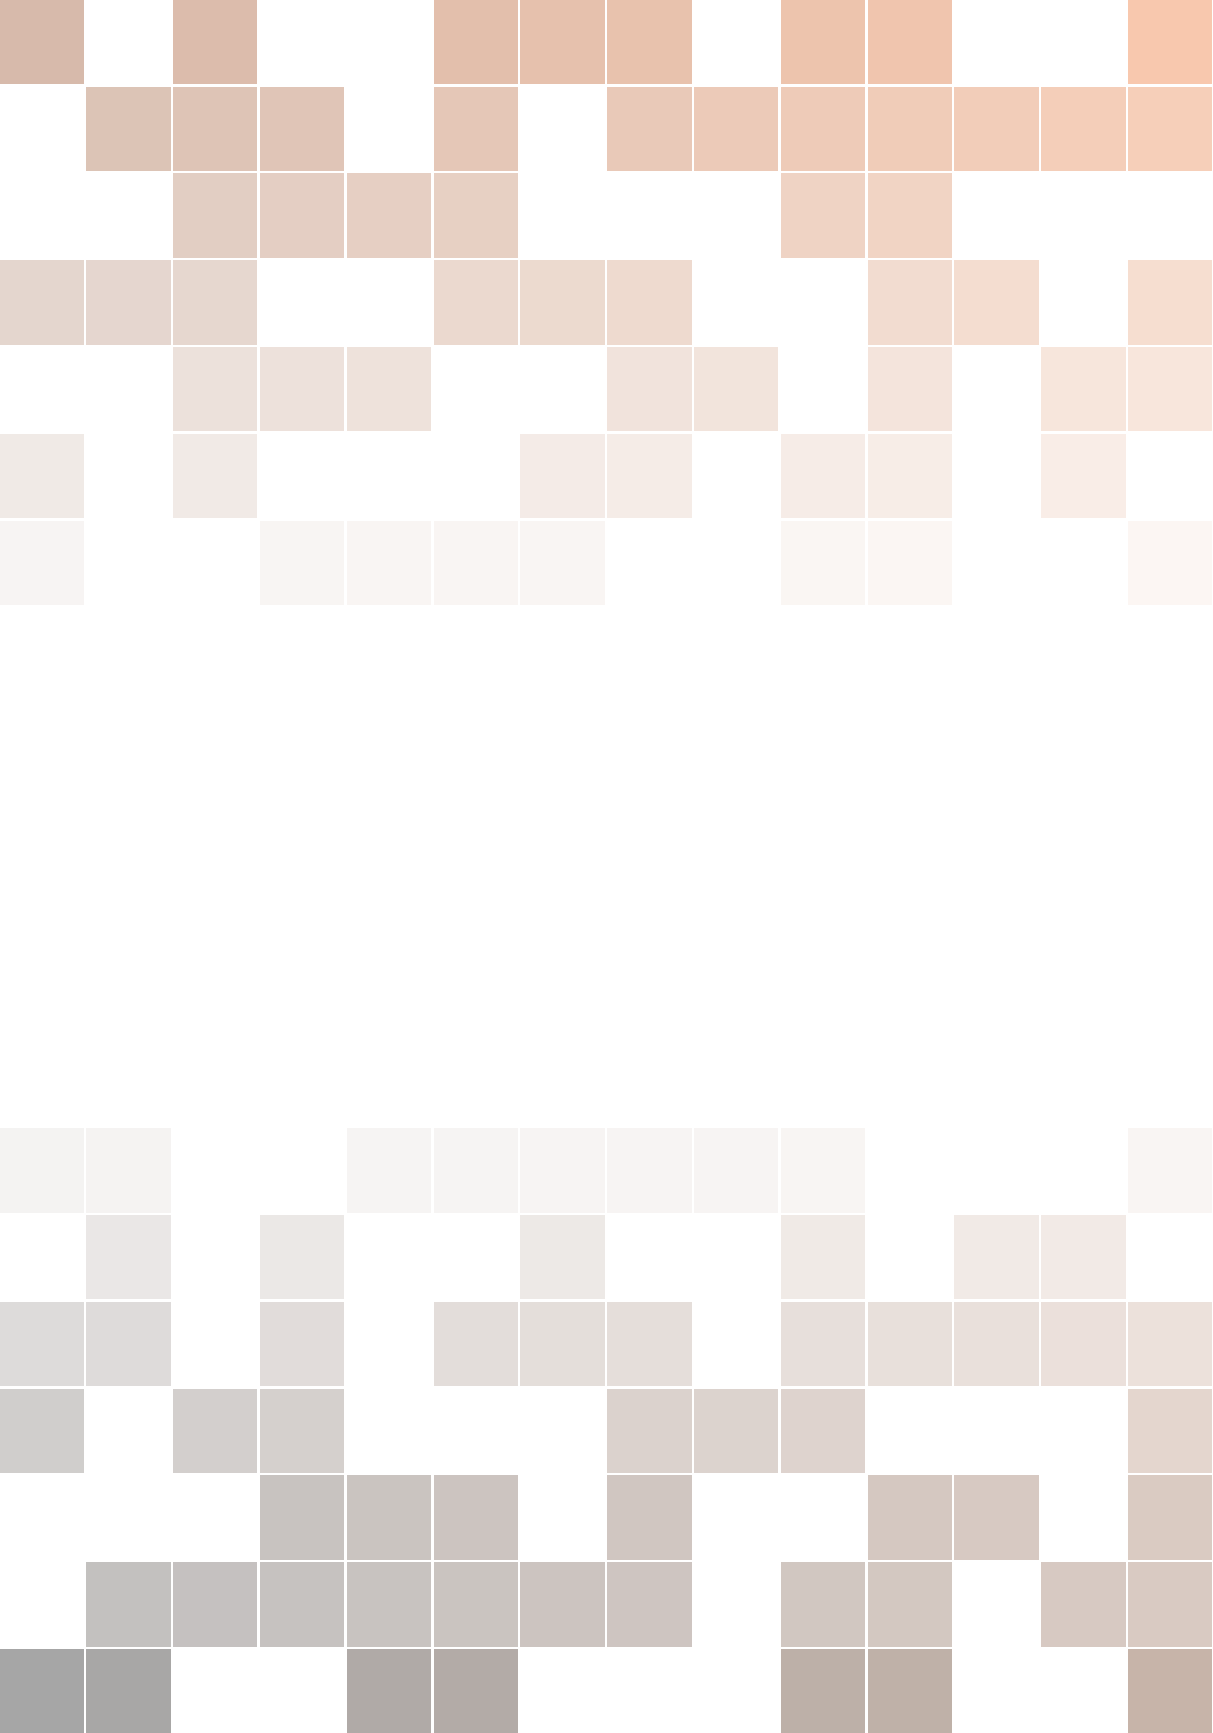
\includegraphics[width=\paperwidth]{background}}; % Background image
\draw[anchor=north] (midpoint) node [fill=ocre!30!white,fill opacity=0.6,text opacity=1,inner sep=1cm]{\Huge\centering\bfseries\sffamily\parbox[c][][t]{\paperwidth}{\centering The Search for a Title\\[15pt] % Book title
{\Large A Profound Subtitle}\\[20pt] % Subtitle
{\huge Dr. John Smith}}}; % Author name
\end{tikzpicture}};
\end{tikzpicture}
\vfill
\endgroup

%----------------------------------------------------------------------------------------
%	COPYRIGHT PAGE
%----------------------------------------------------------------------------------------

\newpage
~\vfill
\thispagestyle{empty}

\noindent Copyright \copyright\ 2013 John Smith\\ % Copyright notice

\noindent \textsc{Published by Publisher}\\ % Publisher

\noindent \textsc{book-website.com}\\ % URL

\noindent Licensed under the Creative Commons Attribution-NonCommercial 3.0 Unported License (the ``License''). You may not use this file except in compliance with the License. You may obtain a copy of the License at \url{http://creativecommons.org/licenses/by-nc/3.0}. Unless required by applicable law or agreed to in writing, software distributed under the License is distributed on an \textsc{``as is'' basis, without warranties or conditions of any kind}, either express or implied. See the License for the specific language governing permissions and limitations under the License.\\ % License information

\noindent \textit{First printing, March 2013} % Printing/edition date

%----------------------------------------------------------------------------------------
%	TABLE OF CONTENTS
%----------------------------------------------------------------------------------------

%\usechapterimagefalse % If you don't want to include a chapter image, use this to toggle images off - it can be enabled later with \usechapterimagetrue

\chapterimage{chapter_head_1.pdf} % Table of contents heading image

\pagestyle{empty} % No headers

\tableofcontents % Print the table of contents itself

\cleardoublepage % Forces the first chapter to start on an odd page so it's on the right

\pagestyle{fancy} % Print headers again

%----------------------------------------------------------------------------------------
%	Contains phonetics, morphology, and syntax.
%----------------------------------------------------------------------------------------

\part{Grammar}

%----------------------------------------------------------------------------------------
%	CHAPTER 1
%----------------------------------------------------------------------------------------

\chapter{Phonology}

\section{Phonetic Inventory}\index{Phonetic Inventory}

\subsection{Consonants}\index{Consonants}

In terms of phonology, Ngujari has a rich consonantal inventory featuring a
large series of coronal consonants (both laminal and apical) and multiple
rhotics. The following table shows the consonants and their orthographic
representation in italics (if different from the IPA).

\begin{table}[h]
\centering
\begin{tabular}{rcccccc}
  & \textbf{bilabial} & \textbf{alveolar} & \textbf{post-alveolar} & \textbf{retroflex} & \textbf{palatal} & \textbf{velar}\\
  \textbf{plosive} & \textipa{p} & \textipa{\|]{t}}\textit{(t)} & & \textipa{\|{]}{\textrtailt}}\textit{(rt)} & & \textipa{k}, \textipa{g}\\
  \textbf{nasal} & \textipa{m} & \textipa{\|]{n}}\textit{(n)} & \textipa{\textsubsquare{n}}\textit{(nn)} & \textipa{\|{]}{\textrtailn}}\textit{(rn)} & & \textipa{N}\textit{(ng)}\\
  \textbf{trill} & & \textipa{\|]{r}}\textit{(rr)} & & & &\\
  \textbf{tap} & & \textipa{\|]R}\textit{(rr)} & & & &\\
  \textbf{fricative} & & & \textipa{Z}\textit{(j)} & & &\\
  \textbf{approximant} & \textipa{w} & & & \textipa{\textturnrrtail}\textit{(r)} & \textipa{j}\textit{(y)} &\\
  \textbf{lateral approximant} & & \textipa{\|]{l}}\textit{(l)} & & \textipa{\|]{\textrtaill}}\textit{(rl)} & &\\
\end{tabular}
\caption{Consonantal Inventory}
\end{table}

\subsection{Vowels}\index{Vowels}

The vowel palette is very restricted, limited to just a, i, and u, as well as
their lengthened versions. The long vowels are contrastive in all locations.
These phonemes are found in the following table.

\begin{table}[h]
\centering
\begin{tabular}{rcc}
& \textbf{front} & \textbf{back}\\
\textbf{high} & \textipa{i}, \textipa{i:} & \textipa{u}, \textipa{u:}\\
\textbf{low} & \textipa{a}, \textipa{a:} &\\
\end{tabular}
\caption{Vowel Inventory}
\end{table}

Orthographically, the short vowels are expressed according to their IPA
representation. Long vowels are simply the short vowel doubled.

The front vowels (i and a) are phonetically tense. Both have a nasalised
allophone.

The back vowel u is divided allophonetically into two sounds: the default u, and
the somewhat centralised \textipa{\"u} which tends towards the \textipa{U} sound
and is accordingly more lax than the default.

\section{Phonotactics}\index{Phonotactics}

\subsection{Syllables and Morae}\index{Syllables}

The structure of Ngujari words is simple, with syllables taking the form CV: one
consonant is followed by one vowel. A root word is usually between two and four
syllables long, plus any affixes which tend to be single-syllable. In addition,
words can be broken into \textit{morae}. A syllable containing a short vowel is
worth one mora, but those containing long vowels are worth two. This distinction
becomes important when dealing with prosody in \autoref{prosody}.


\subsection{Vowels}

The \textit{u} phoneme becomes centralised following some bilabial consonants p, m, and w.

\begin{quote}
\phonc{u}{\textipa{\"u}}{\oneof{p \phold\\ m \phold\\ w \phold}}
\end{quote}

The i and a phonemes are nasalised before alveolar and post-alveolar nasals.

\begin{quote}
\begin{multicols}{2}
\phonc{i}{\textipa{\~i}}{\oneof{\phold \textipa{\|]{n}}\\ \phold
    \textipa{\textsubsquare{n}}}}

\phonc{a}{\textipa{\~a}}{\oneof{\phold \textipa{\|]{n}}\\ \phold
    \textipa{\textsubsquare{n}}}}
\end{multicols}
\end{quote}

\subsection{Consonants}

\subsubsection{Rhotics}

The alveolar trill becomes a tap if it follows a short vowel, while remaining
apicalised.

\begin{quote}
\phonl{\textipa{\|]r}}{\textipa{\|]R}}{\oneof{a\\u\\i}}
\end{quote}

The retroflex approximant \textipa{\textturnrrtail} disappears between identical
regular vowels, forming one lengthened vowel.

\begin{quote}
\phonc{\textipa{\textturnrrtail}}{\o}{\oneof{a \phold a\\ u \phold u\\ i \phold i}}
\end{quote}

\subsubsection{Voicing}

The voicing process is relatively new to the language, and accordingly not much
variation is present. Generally, plosives are becoming initially voiced.
However, in practice the voiced plosive g is the only new voiced consonant
sufficiently formed to be included as an individual phoneme; the rest are in the
process of undergoing the differentiation. In the case of the \textipa{\|]{t}}
phoneme, only the alveolar form undergoes voicing, as the retroflex cannot begin
a word.

\begin{quote}
\begin{multicols}{3}
\phonl{k}{g}{\^{}}

\phonl{p}{\textipa{\v*p}}{\^{}}

\phonl{\textipa{\|]{t}}}{\textipa{\t*p}}{\^{}}\footnote{The phoneme remains
  apical, but this cannot be expressed in IPA.}
\end{multicols}
\end{quote}

\subsection{Historical Sound Changes}\index{Historical Sound Changes}

Ngujari differs phonologically from Proto-Pama-Nyungan only slightly. The
following is a list of sound changes that have occured:

\begin{itemize}
\item Apicalised post-alveolar plosive (\textipa{\textsubsquare{t}}) becomes
  voiced post-alveolar fricative (\textipa{Z}).
\item Apicalised alveolar trill (\textipa{\|]r}) becomes apicalised alveolar tap
  (\textipa{\|]R}) immediately following regular vowels.
\item Retroflex approximant (\textipa{\textturnrrtail}) disappears between
  identical regular vowels, forming one lengthened vowel.
\item Apicalised alveolar lateral approximant (\textipa{\|]l}) disappears from
  the end of words.
\end{itemize}

A major difference occurs in the case of lengthened vowels, which can
differentiate words in all positions, rather than just the first syllable as in
the protolanguage.

\section{Prosody}\index{Prosody}\label{prosody}

Ngujari has a rich prosodic system incorporating stress, intonation, and tempo.
Stress is dealt with here, but intonation and tempo are left to Part 2 in the
discussion on pragmatics.

\subsection{Stress}
Stress follows a simple process. The primary stress is placed on the second mora
of the word. If that mora is part of the first syllable (i.e. the first syllable
has a long vowel rendering it bimoraic), the first syllable is stressed.
Secondary stress is then placed on morae at even intervals, on the 4th, 6th,
etc. However, if the secondary stress would fall on the second mora of a
bimoraic syllable, it is skipped.

\chapter{Morphology}

\section{Nouns}\index{Nominal Morphology}

\subsection{Gender}\index{Gender}

Ngujari has four genders: child, adult, elder (grouped together as animate), and
inanimate. Gender is assigned semantically and changes the morphosyntactic
alignment of the sentence as well as posessives.

The animate gender is given to people, animals, and Dreamtime figures. For
example, \textit{Yawirra}, the concept of the Land, is considered animate. The
inanimate gender applies to all other nouns.

Within the animate there are three genders, each representing a different stage
in life. This distinction is important in areas such as pronouns, but not in
others, like verbal inflection. An animate noun is assigned to a stage based on
their social position. Those who are yet to undergo the adulthood ceremony
(those under roughly 14 in the case of females and 16 in the case of males) are
assigned the child gender, while those who have become elders receive the elder
gender. All other ages are grouped into the adult gender.

\subsection{Cases}\index{Cases}

Ngujari has eight nominal cases, with three indicating the morphosyntactic
alignment and five others. Cases are indicated by single-syllable suffixes, as
indicated in the following table.

\begin{table}[h]
\centering
\begin{tabular}{lcc}
\textbf{case} & \textbf{abbreviation} & \textbf{suffix}\\
ergative & \textsc{erg} & -\\
nominative & \textsc{nom} & -wa\\
accusative & \textsc{abs} & -rru\\
instrumental & \textsc{ins} & -ma\\
comitative & \textsc{com} & -yii\\
orientative & \textsc{ori} & -rni\\
revertive & \textsc{rev} & -nga\\
locative & \textsc{loc} & -ru\\
\end{tabular}
\caption{Case Suffixes}
\end{table}

For more details on the three alignment cases, see \ref{sec:alignment} (pg.
\pageref{sec:alignment}). The remaining five cases operate as follows:

\begin{description}
\item[instrumental] The instrumental case is used when discussing a *means*,
  roughly equivalent to the English ``by means of''. For example, when speaking
  of killing a fish using a spear, a Ngujari speaker will place ``spear'' in the
  \textsc{INS} case.
\item[comitative] The comitative case is equivalent to ``in the presence of'',
  or ``with'', and specifies that the noun was present at the moment spoken of.
\item[orientative] The orientative case is used to specify that something is
  facing towards the noun. It is often used with the meaning of ``heading
  towards''.

  aux 2s-ERG camp-ORI togo-an-2nd.

  You are heading towards the camp.

\item[revertive] The revertive case is used to specify that something is
    oriented away from the noun. It can be used with the meaning of ``heading
    away from''.

  aux 3pl-an-NOM 3s-an-REV togo-an-3rd.

  They are heading away from her.

  It can also be used in asserting falsehood.

  aux-remote 3s-an-ERG knowledge-NOM valence1->2 tolook-an-3rd.

  He used to look away from knowledge / he used to be incorrect.

\item[locative] The locative case is used to specify a location, and can take
  the place of a preposition such as ``in'' or ``at''. This means that ``she is
  at the house'' is equivalent to ``she is [house] (\textsc{LOC})''. The
  locative suffix *-ru* becomes a long u if placed after a word ending in a
  short u.

\end{description}

An example of the use of these cases is found in the following table, which
shows the declensions of the noun \textit{naju}, or ``rock''.

\begin{table}[h]
\centering
\begin{tabular}{lll}
\textbf{case} & \textbf{word} & \textbf{meaning}\\
ergative & naju & -\\
nominative & najuwa & -\\
accusative & najurru & -\\
instrumental & najuma & ``using the rock''\\
comitative & najuyii & ``in the presence of the rock''\\
orientative & najurni & ``oriented towards the rock''\\
revertive & najunga & ``orientated away from the rock''\\
locative & najuu & ``at the rock''\\
\end{tabular}
\caption{Examples of Nominal Case Declensions}
\end{table}

\section{Plurality}\index{Plurality}

Plurals are formed through reduplication, with the declined noun repeated twice.
For example, *najurru* ("rock", in the absolutive case), would be pluralised as
*najurru-najurru*.

There are two forms of plural, which differentiate dual and non-dual plurality.
The default case is non-dual, but the clitic *ka* following the reduplicated
noun indicates the dual form.

\section{Verbs}\index{Verbal Morphology}

Verbs in Ngujari are found in three classes, each with a specified stem ending
and auxiliary form. Verb roots lack a final consonant, meaning they must be
conjugated in order to appear in speech. Class does not have any semantic
impact; it changes only the morphology of the verb.

The three classes are:

\begin{table}[h]
\centering
\begin{tabular}{lccc}
\textbf{class} & \textbf{ending} & \textbf{auxiliary} & \textbf{negative particle}\\
\textbf{first} & -rr & kuurl & tu\\
\textbf{second} & -j & ngiy & ti\\
\textbf{third} & -nn & wann & wuu\\
\end{tabular}
\caption{Verb Classes}
\end{table}

To conjugate a verb, both it and its auxiliary must be declined. The verb itself
is conjugated in agreement, with the gender and person of the subject indicated
as affixes. The auxiliary is declined to indicate tense and mood.

\subsection{Tense and Mood}\index{Tense and Mood}

There are four tenses: remote past, past, present, and future. There is no
distinction drawn between the perfective and imperfective aspects, meaning
contextual clues are vital for understanding.

Present is considered the default tense, and is accordingly unmarked for first
and second class verbs (but not third). It usually indicates those events which
are happening in the moment of utterance, but it can also be used as a
rudimentary form of a near-past tense, applying to actions that were completed
the same day as the utterance.

Past and remote past are marked for all verb classes and indicate an event that
was completed in the past. Choice between the two can be somewhat arbitrary, but
in general remote past is used when recounting handed-down stories or the events
of ancestral times, whereas basic past refers to events in the time period of
the speaker. If the event has not yet finished, the present tense is used.

Future is again marked for all classes. All events which are yet to take place
are assigned the future tense.

There are five moods that a verb can optionally be conjugated for:

\begin{itemize}
\item subjunctive
\item weak imperative
\item strong imperative
\item gnomic
\item dubitative
\end{itemize}

\begin{description}

\item[subjunctive] The subjunctive mood is an irrealis mood which broadly
  signifies abstractness and is used in a number of ways:

  \begin{enumerate}
      \item Speculation
      \item Conditional
      \item Desires
      \item Purposive
  \end{enumerate}

\item[imperative] The imperative mood is used for suggestions and commands. The
  weak form raises an idea without indicated an order, similar to the English
  ``let's go'', whereas the strong form signifies a command, such as ``Leave!''.

\item[gnomic] The gnomic mood states unequivocal facts or ideas. The statement
  must be truly uncontentious to fit into the gnomic mood, such as ``fire is
  real''.

\item[dubitative] The dubitative mood indicates situational possibility, in that
  the speaker acknowledges the possibility of an action but is unsure as to
  whether it occurs, as in English ``might''.

\end{description}

\subsection{Verbal Conjugation Tables}

\begin{table}[h]
\centering
\begin{tabular}{lcccc}
\textbf{class} & \textbf{child} & \textbf{adult} & \textbf{elder} & \textbf{inanimate}\\
first & uu & u & iiwa & a\\
second & awuu & awu & iwu & a\\
third & arruu & u & iwu & aa\\
\end{tabular}
\caption{Gender of Subject}
\end{table}

\begin{table}[h]
\centering
\begin{tabular}{lccc}
\textbf{class} & \textbf{1st} & \textbf{2nd} & \textbf{3rd} \\
first, second & -           & ku          & nni    \\
third & -           & ku          & ni    \\
\end{tabular}
\caption{Person of Subject}
\end{table}

\subsection{Auxiliary Conjugation Tables}

\begin{table}[h]
\centering
\begin{tabular}{lcccc}
\textbf{class} & \textbf{remote past} & \textbf{past} & \textbf{present} & \textbf{future}\\
first & arlu & a & --- & aa \\
second & arlu & a & --- & aju\\
third & una & uma & uu & uuki\\
\end{tabular}
\caption{Tense}
\end{table}

\begin{table}[h]
\centering
\begin{tabular}{lccccc}
\textbf{class} & \textbf{subjunctive} & \textbf{weak imperative} & \textbf{strong imperative} & \textbf{gnomic} & \textbf{dubious}\\
first &  tiru & yii & ju & nga & tila\\
second & tirlu & yii & yuu & nga & ti\\
third &  tirlu & yii &  aru & nga & ti\\
\end{tabular}
\caption{Mood}
\end{table}

\subsection{Valence Modification}\index{Valence Modification}

The verbal system of Ngujari allows for many different valences through
derivations of base verbs. Each verb root has its own \textit{default valence},
between avalent (0 arguments) to quadrivalent (4 arguments). Furthermore, each
verb has a \textit{minimum valence} and \textit{maximum valence}, i.e. the
extent that valency can be modified while still modifying the verb's meaning,
rather than imparting additional information. The maximum valence is never above
4.

For example, the verb \textit{wurr} has a default valence of 0, in which case it
means ``it is electrically storming''. However, modifying its valence to 1
allows it to mean ``to be struck by lightning'', and a valence of 2 allows it to
mean ``to strike''. Therefore, it has a minimum valence of 0 and maximum valence
of 2.

Valence modification occurs through special particles, which are found in the
following table:

\begin{table}[h]
\centering
\begin{tabular}{lllllll}
                                  &   & \multicolumn{5}{c}{\textbf{target}} \\
                                  &   & 0     & 1     & 2   & 3     & 4     \\
\multirow{5}{*}{\textbf{default}} & 0 & ---   & wi    & ji  & murnu & yurnu \\
                                  & 1 & wi    & ---   & naa & naki  & mu    \\
                                  & 2 & waa   & ka    & --- & naa   & naki  \\
                                  & 3 & wangu & waa   & ka  & ---   & naa   \\
                                  & 4 & wirru & wangu & waa & ka    & ---
\end{tabular}
\caption{Valence Modification Particles}
\end{table}

The prime function of derived valences is to change the meaning of the verb. In
this case, the new meaning must be learned, as well as the noun cases it
accepts.

\section{Adjectives and Adverbs}\index{Adjectives and Adverbs}

Adjectives are inflected into two categories: attribute and predicate. The
attributive form is unmarked, and can be used directly in noun phrases to
describe the noun. The predicate form can only be used in predicative phrases,
and is declined according to the gender and person of the noun it applies to.

To decline a predicate adjective, the final vowel is dropped and the same
declensions as class one verbs are applied.

Adverbs are not declined, but are divided semantically into the classes manner
(hastily, carefully) and temporal (last week, yesterday). The class of an adverb
loosely determines its position in a phrase. See \ref{adverbposition} for more
information.

\chapter{Pronouns}

\section{Personal}\index{Personal Pronouns}

Personal pronouns differ in three dimensions: person, plural, and gender. All
decline in the same way as regular nouns to indicate case. The following tables
list the pronouns:

\begin{table}[h]
\centering
\begin{tabular}{lccc}
 & \textbf{singular} & \textbf{dual} & \textbf{plural}\\
 \textbf{1st person} & jana & janna & juu\\
 \textbf{2nd person} & kurru & kunii & kurlu\\
 \textbf{3rd person} & nnarta & nnaja & nni\\
\end{tabular}
\caption{Child Personal Pronouns}
\end{table}

\begin{table}[h]
\centering
\begin{tabular}{lccc}
 & \textbf{singular} & \textbf{dual} & \textbf{plural}\\
 \textbf{1st person} & wa & ja & waya\\
 \textbf{2nd person} & ku & kuna & kuu\\
 \textbf{3rd person} & nna & nnara & nnaa\\
\end{tabular}
\caption{Adult Personal Pronouns}
\end{table}

\begin{table}[h]
\centering
\begin{tabular}{lccc}
 & \textbf{singular} & \textbf{dual} & \textbf{plural}\\
 \textbf{3rd person} & nnu & nnuka & nnunnu\\
\end{tabular}
\caption{Inanimate Personal Pronouns}
\end{table}

When speaking of a mob's elders, a personal pronoun is never used. The elder is
always referred to by their honorific title.

\section{Possessive}

Possessive pronouns are formed through a suffix placed on the relevant personal
pronoun, but only for the child and adult genders. For possession by elders, see
\ref{tribepos}. Inanimate objects cannot be possessive. For a child, the suffix
is \textit{ra} in first and second person and \textit{raa} in third person. For
an adult, the suffix is \textit{lu} for all persons.

\section{Interrogative}\index{Interrogative Pronouns}

The interrogative pronouns are strongly affected by case, particularly in the
case of location and time. The basic pronouns are detailed in the following
table:

\begin{table}[h]
\centering
\begin{tabular}{lc}
 \textbf{meaning} & \textbf{word}\\
 where & kiru\\
 when & tuu\\
 who, what & pii\\
 how & piima\\
 why & wiirtak\\
 how many & kirta\\
\end{tabular}
\caption{Interrogative Pronouns}
\end{table}

It is interesting to note that ``how'' is the same as ``what'' placed in the
instrumental case. The orientative and revertive cases can be applied to
\textit{kiru} (``where''), forming \textit{kirurni} (``whither/to where'') and
\textit{kirunga} (``whence/from where''), as well as to \textit{tuu} (``when''),
forming \textit{tuurni} (``to when'') and \textit{tuunga} (``from when'').

\section{Demonstrative}\index{Demonstrative Pronouns}

One set of demonstrative pronouns covers both proximal and distal objects.
Distinctions can be made in some cases between both gender and number. The
pronouns are found in the following table:

\begin{table}[h]
\centering
\begin{tabular}{lccc}
 \textbf{meaning} & \textbf{singular} & \textbf{dual} & \textbf{plural}\\
 there & naarla & naarla & naarla\\
 then & yaji & yaji & yaji\\
 that (animate) & yanna & yannara & yannaa\\
 that (inanimate) & yannu & yannuka & yannunnu\\
\end{tabular}
\caption{Demonstrative Pronouns}
\end{table}

Again, the pronouns \textit{naarla} and \textit{yaji} can assume the orientative
and revertive cases.

\section{Indefinite}\index{Indefinite Pronouns}

The regular indefinite pronouns are formed through modifying the interrogative
pronouns by appending the correct word, representing number. These words are
listed in the following table:

\begin{table}[h]
\centering
\begin{tabular}{lc}
 \textbf{number} & \textbf{word}\\
 none & nnayi\\
 singular & junga\\
 dual & marri\\
 plural & munaa\\
 all & nnaya\\
\end{tabular}
\caption{Indefinite Pronouns}
\end{table}

For example, ``everyone'' would be expressed as \textit{pii-nnaya} and ``some
two locations'' as \textit{kiru-marri}.

\chapter{Syntax}

\section{Alignment}\index{Morphosyntactic Alignment}

The alignment of Ngujari depends on whether the noun in question is an animate
pronoun or not. For clauses with exclusively animate pronouns, the alignment is
nominative-accusative, but otherwise it is ergative-nominative (i.e. the
transitive patient and intransitive object are marked nominative and the
transitive agent is marked ergative). This system applies only to intransitive
and transitive verbs. For higher valencies, formed through \ref{valencemod}, the
extra arguments are assigned cases semantically.

\section{Verb Phrases}\index{Verb Phrases}

\begin{definition}[Verb Phrase]
~\\
\textsc{vp = aux [neg] np(s) [adv(s)] [val] v}
\end{definition}

Verb phrases can be as simple as a single avalent verb, such as in ``it's raining'', or as complex as a tetravalent causative.

In the prototypical verb clause, the following rules govern word order:

\begin{enumerate}
\item The verb's auxiliary appears at the beginning.
\item The verb itself appears at the end.
\item Valence modifiers appear immediately before the verb.
\end{enumerate}

The following examples illustrate basic verb phrases:

\begin{sentence}
\shortex{5}
{\bfseries k-i & \bfseries wa-j & \bfseries kurru-l & \bfseries ji &
  \bfseries wurr-u-\o.}
{strike.\textsc{aux-pres} & 1\textsc{s-nom} & 2\textsc{s-ACC} & \textsc{0.val.2} & electrically.storm-\textsc{an}-\textsc{1st}}
{\textit{I strike you.}}

\shortex{4}
{\bfseries wann-uma & \bfseries maaju-maaju-j & \bfseries ka & \bfseries jinn-u-m.}
{see.\textsc{aux-pst} & kangaroo-\textsc{pl-nom} & \textsc{2.val.1} & eat-\textsc{an-3rd}}
{\textit{The kangaroos ate/were eating.}}
\end{sentence}

Noun phrases tend to appear in order of importance to the statement as judged by
the speaker.

\section{Noun Phrases}\index{Noun Phrases}

\begin{definition}[Verb Phrase]
~\\
\textsc{np = [adj(s)-attr] n [rel(s)]}
\end{definition}

A noun phrase consists of one noun, declined by case, and any number of
adjectives and relative clauses. The noun tends to be placed first, followed by
adjectives, although this can be inverted or even mixed according to pragmatic
considerations. However, relative clauses always succeed the noun and
adjectives.

\begin{sentence}

\shortex{3}
{\textbf{birru-\o} &\textbf{birruku} &\textbf{miinna} }
{sea-\textsc{ERG} &blue &big}
{\textit{vast blue sea}}

\shortex{3}
{\textbf{kanaama} &\textbf{yirlirna-j} &\textbf{gu} }
{woven &basket-\textsc{NOM} &small}
{\textit{small woven basket}}

\end{sentence}

\section{Relative Clauses}\index{Relative Clauses}\label{relativeclauses}

\begin{definition}[Relative Clause]
~\\
\textsc{vp = aux [neg] np(s) [adv(s)] [val] v}\\
$\Rightarrow$ \textsc{rc = aux [neg] v [val] [adv(s)] np(s)}
\end{definition}

Relative clauses are \textit{adjoined} to the noun phrase. The clause undergoes
a transformation from the standard verb phrase by moving the verb to the
position immediately following the auxiliary. The valency modifier is free to be
placed anywhere among the remaining noun phrases and adverbs, but typically
follows the verb.

If the head noun is a patient of the relative clause, the verb of the relative
clause has its valence reduced by one.

\begin{sentence}
\shortex{5}
{\textbf{wiingu-\o} &\textbf{k-a} &\textbf{pirr-u-\o} &\textbf{ka} &\textbf{wa-j}}
{man-\textsc{erg} &\textsc{aux}-\textsc{pst} &see-\textsc{an}-1\textsc{st} &2.\textsc{val}.1 &1s-\textsc{nom}}
{\textit{the man that I saw}}
\end{sentence}

If the head noun is the agent, a pronoun is used inside the relative clause to
refer back to it.

\begin{sentence}
\shortex{6}
{\textbf{j-a} &\textbf{Wuurna-\o} &\textbf{nn-uuki-ti} &\textbf{yann-u-mi} &\textbf{nna-j} &\textbf{jurlu-l}}
{say.\textsc{aux}-\textsc{pst} &Wuurna-\textsc{erg} &\textsc{aux}-\textsc{fut}-\textsc{dub} &catch-\textsc{an}-3\textsc{rd} &3s-\textsc{nom} &turtle-\textsc{acc}}
{}\\
\shortex{3}
{\textbf{wa-j} &\textbf{ka} &\textbf{naj-u-m} }
{1s-\textsc{nom} &3.\textsc{val}.2 &say-\textsc{an}-3\textsc{rd} }
{\textit{Wuurna, who might catch a turtle, spoke to me.}}

\end{sentence}

\subsection{Adverbial Phrases}\index{Adverbial Phrases}
\label{advsyntax}

Temporal adverbs, which specify the time an action takes place, tend to appear
following the noun.

\begin{sentence}
\shortex{6}
{\textbf{k-a} &\textbf{jana-\o} &\textbf{jari-rn} &\textbf{wiirr-uu-\o} &\textbf{yuurli-rna} &\textbf{ma} }
{go.\textsc{aux}-\textsc{pst} &1s.\textsc{ch}-\textsc{erg} &beach-\textsc{loc} &go-\textsc{ch}-1\textsc{st} &day-\textsc{rev} &one }
{\textit{Yesterday, I [a child] went to the beach.}}
\end{sentence}

Manner adverbs, which specify the manner in which the action was conducted,
usually appear directly before the noun.

aux(topickup)-weakimp 1pl-ERG clothes(pl)-NOM quickly pickup-an-3rd.

We should pick up the clothes quickly.

However, both can occupy different positions inside the verb phrase if the
speaker desires it.

\section{Predicates}\index{Predicates}

There are three cases for predicates: adjectival, nominal, and locational.

In an adjectival predicative phrase a verb is not normally required. The noun is
assigned the same tense as it would be were it the argument to an intransitive
verb, while the adjective assumes its predicative inflection.

\begin{sentence}
\shortex{2}
{\textbf{puurna-j} &\textbf{birruku-ku} }
{sky-\textsc{nom} &blue-\textsc{an} }
{\textit{The sky is blue.}}
\end{sentence}

Sometimes, the comitative case is used along with the verb ``to be'' in an
adjectival phrase, usually when describing a changeable state.

berry-NOM freshness-COM.

the berry is with freshness/is fresh.

In a nominal predicative phrase, the verb ``to be'' is used. The predicate noun
is declined as verb's object.

\begin{sentence}
\shortex{4}
{\textbf{ngarr-i} &\textbf{wa-\o} &\textbf{gajangu-j} &\textbf{ngurr-u-\o} }
{be.\textsc{aux}-\textsc{pres} &1\textsc{s}-\textsc{erg} &teacher &be-\textsc{an}-1\textsc{st} }
{\textit{I am a teacher.}}
\end{sentence}

In a locational predicative phrase, the verb ``to be'' is still used, but the
predicate location is declined in the locative case.

\begin{sentence}
\shortex{4}
{\textbf{k-i} &\textbf{wurlki-\o} &\textbf{kirujunga-\o} &\textbf{ngurr-a-m} }
{be.\textsc{aux}-\textsc{pres} &village-\textsc{erg} &somewhere-\textsc{loc} &be-\textsc{inan}-3\textsc{rd} }
{\textit{The village is somewhere.}}
\end{sentence}

\section{Possession}\index{Possession}

\subsection{Alienable}

To indicate alienable possession (possession that is not permanent or subject to
change), the locative case is used in conjunction with the verb ``to be''. The
possessed noun appears in the locative case as the subject of the transitive
form of ``to be'', with the possessor appearing as the object in the usual case.

\begin{sentence}
\shortex{4}
{\textbf{ngarr-i} &\textbf{mulu-mulu-ka-rn} &\textbf{mungu-j} &\textbf{ngurr-a-m} }
{be.\textsc{aux}-\textsc{pres} &deadfish-\textsc{pl}-\textsc{dual}-\textsc{loc} &woman-\textsc{nom} &be-\textsc{inan}-3\textsc{rd} }
{\textit{The woman has two dead fish.}}
\end{sentence}

\subsection{Inalienable}

Inalienable possession (possession that is unequivocal) is indicated simply
through the use of the verb ``to have''.

\begin{sentence}
\shortex{5}
{\textbf{garr-aa-nga} &\textbf{ngungu-j} &\textbf{jarta-l} &\textbf{ka} &\textbf{gurr-u-\o} }
{have.\textsc{aux}-\textsc{fut}-\textsc{gno} &mob-\textsc{nom} &homeland-\textsc{acc} &3.\textsc{val}.2 &have-\textsc{an}-1\textsc{st} }
{\textit{Our mob will always have a homeland.}}
\end{sentence}

\subsection{Pronominal}

A noun phrase can be indicated as possessed through the use of a possessive
pronoun as an adjective.

aux-past 3pl-an-ERG face-NOM beautiful his admire-an-3rd

they admired his beautiful face

\begin{sentence}
\shortex{6}
{\textbf{nn-uma} &\textbf{nnaa-\o} &\textbf{waju-j} &\textbf{yurni} &\textbf{nna-lu} &\textbf{giinn-u-m} }
{admire.\textsc{aux}-\textsc{pst} &3\textsc{pl}.\textsc{an}-\textsc{erg} &face-\textsc{nom} &beautiful &3\textsc{s}.\textsc{an}-\textsc{pos} &admire-\textsc{an}-3\textsc{rd} }
{\textit{They admired his beautiful face.}}
\end{sentence}

In Ngujari culture, an object can be owned by a mob as a whole. Only inanimate
objects may be possessed by a mob (with the exception of areas of land).
Possession is indicated by the particle \textit{tuu}, which appears before the
noun. To specify the possessing mob, the mob's name is placed immediately after
the particle. The regular name is used by members of the possessing mob, but the
honorific name is used for possessions of others. For example, the particle for
something owned by the Wujanga mob would be \textit{tuu-Wujanga} for a member or
\textit{tuu-Wujarra} for an outsider.

\begin{sentence}
\shortex{5}
{\textbf{nn-i-ju} &\textbf{waya-\o} &\textbf{tuu-Gurnu} &\textbf{jaku} &\textbf{nnalu-j} }
{protect.\textsc{aux}-\textsc{strimp} &1\textsc{pl}-\textsc{erg} &\textsc{pos}-\textsc{g}urnu &precious &land-\textsc{nom} }
{\textit{}}
\shortex{3}
{\textbf{muu-ma} &\textbf{naa} &\textbf{tinn-u-\o} }
{spirit-\textsc{inst} & 2.\textsc{val}.3 & protect-\textsc{an}-1\textsc{st} }
{\textit{We must protect our [the Gurnu mob's] precious land with vigour.}}
\end{sentence}

\section{Verbal Constructions}\index{Verbal Constructions}

\subsection{Interrogative}\index{Interrogative}

\subsubsection{Polar Questions}

Polar questions are syntactically the same as a factual statement, except they
are expressed with a rising tone at the beginning of the question.

\begin{sentence}
\shortex{4}
{\textbf{nn-uuki} &\textbf{kupa-kupa-\o} &\textbf{gaypa-gaypa-rn} &\textbf{narnn-u-m?} }
{\textglobrise fly.\textsc{aux}-\textsc{fut} &bird-\textsc{pl}-\textsc{erg} &mountain-\textsc{pl}-\textsc{loc} &fly-\textsc{an}-3\textsc{rd} }
{\textit{Will the birds fly to the mountains?}}
\end{sentence}

\subsubsection{Non-Polar Questions}

One way of forming a non-polar question is using an interrogative pronoun as a
verb's argument, with no syntactic change taking place.

\begin{sentence}
\shortex{6}
{\textbf{kiru} &\textbf{ngarr-i} &\textbf{wumpa-j} &\textbf{j-i} &\textbf{palyaj-a-m} &\textbf{nnu-\o} }
{where &be.\textsc{aux}-\textsc{prs} &path-\textsc{nom} &leadto.\textsc{aux}-\textsc{prs} &leadto-\textsc{inan}-3\textsc{rd} &3\textsc{s}.\textsc{inan}-\textsc{erg} }
{}
\shortex{2}
{\textbf{wurlki-j} &\textbf{ngurr-a-m} }
{village-\textsc{nom} &be-\textsc{inan}-3\textsc{rd} }
{\textit{Where is the path that leads to the village?}}
\end{sentence}

To question a certain word in a statement, the particle *yuu* can be placed
before the word.

\begin{sentence}
\shortex{5}
{\textbf{k-aa} &\textbf{yuu-nnara-\o} &\textbf{nurtwu-j} &\textbf{panwa-rnu} &\textbf{mirr-uu-m} }
{bring.\textsc{aux}-\textsc{fut} &\textsc{int}-3\textsc{dual}.\textsc{an}-\textsc{erg} &food-\textsc{nom} &fire-\textsc{ori} &bring-\textsc{ch}-3\textsc{rd} }
{\textit{Will \textbf{those two children} bring the food to the fire?}}

\shortex{5}
{\textbf{nn-i} &\textbf{wa-\o} &\textbf{yuu-gurlurni} &\textbf{parnti-j} &\textbf{jinn-u-mi} }
{eat.\textsc{aux}-\textsc{pres} &3\textsc{s}-\textsc{erg} &\textsc{int}-fresh &kangaroomeat-\textsc{nom} &eat-\textsc{an}-3\textsc{rd} }
{\textit{Is he eating \textbf{fresh} kangaroo meat?}}
\end{sentence}

\subsection{Comparative}\index{Comparative Phrases}

Ngujari contains locational-type comparatives. This means that the
\textit{standard} noun, or the noun to be judged against, is marked in the
revertive case. Comparatives do not use a verb, and are always positive (i.e.
more adjective than the standard). The adjective is in the predicative
inflection.

\begin{sentence}
\shortex{3}
{\textbf{nna-j} &\textbf{wa-rna} &\textbf{yam-u} }
{3\textsc{s}-\textsc{nom} &1\textsc{s}-\textsc{rev} &tall-\textsc{an} }
{\textit{He is taller than me.}}
\end{sentence}

For comparatives in relative clauses, the adjective is fronted and is followed
by the arguments.

\begin{sentence}
\shortex{5}
{\textbf{k-a} &\textbf{nnalji-\o} &\textbf{junn-u} &\textbf{nna-\o} &\textbf{wiinguurki-rna} }
{win.\textsc{aux}-\textsc{pst} &dingo-\textsc{erg} &fast-\textsc{an} &3\textsc{s}-\textsc{erg} &boy-\textsc{rev} }
{\textit{}}
\shortex{3}
{\textbf{yuki-j} &\textbf{ka} &\textbf{giirr-u-m} }
{race-\textsc{nom} &2.\textsc{val}.1 &win-\textsc{an}-3\textsc{rd} }
{\textit{The dingo, who is faster than the boy, won the race.}}
\end{sentence}

\subsection{Conditional}\index{Conditional Phrases}

There are two types of conditionals: implicative and predictive. The protasis
(condition) and apodosis (outcome) are modified in different ways.

\begin{description}
\item[implicative] The conditional is a universal truth. Whenever the condition
  is true, the outcome is also true.
\item[predictive] The conditional is a prediction. If the condition occurs, the
  outcome will occur.
\end{description}

To form both conditionals, the condition verb phrase appears first, followed
immediately by the outcome verb phrase. There is no morpheme with equivalent
meaning to ``if''. However, the outcome is always placed in the subjunctive
mood and the present tense.

In an implicative conditional, the condition is given the gnomic mood. The
statement must therefore follow the usual rules of the gnomic, in that it must
state an undisputable truth. The condition is always in the present tense.

\begin{sentence}
\shortex{5}
{\textbf{k-i-nga} &\textbf{kunii-\o} &\textbf{mu-rn} &\textbf{naa} &\textbf{yarr-uu-n} }
{fall.\textsc{aux}-\textsc{prs}-\textsc{gno} &2\textsc{dual}.\textsc{ch}-\textsc{erg} &water-\textsc{loc} &1.\textsc{val}.2 &fall-\textsc{ch}-2\textsc{nd} }
{\textit{}}
\shortex{4}
{\textbf{j-i-tirlu} &\textbf{kunii-j} &\textbf{ka} &\textbf{mulj-awuu-n} }
{wet.\textsc{aux}-\textsc{prs}-\textsc{sbjv} &2\textsc{dual}-\textsc{ch}-\textsc{nom} &2.\textsc{val}.1 &wet-\textsc{ch}-2\textsc{nd} }
{\textit{If you two fall in the water, you will both get wet.}}
\end{sentence}

In a predictive conditional, the condition is usually not given a mood.
However, if the phrase is counterfactual, in that the condition is not seen as
likely, the conditon occurs in the dubitative mood. Usually, the condition
will be in the future tense.

\begin{sentence}
\shortex{5}
{\textbf{nn-uuki} &\textbf{palwuuwa-j} &\textbf{ka} &\textbf{girnn-aa-mi} &\textbf{k-i}}
{break.\textsc{aux}-\textsc{fut} &branch-\textsc{nom} &2.\textsc{val}.1 &break-\textsc{inan}-3\textsc{rd} &strike.\textsc{aux}-\textsc{pres}  }
{\textit{}}

\shortex{4}
{\textbf{yannu-\o} & \textbf{nna-j} &\textbf{ji} &\textbf{wurr-a-rn} }
{\textsc{dem}.\textsc{sg}.\textsc{inan}-\textsc{erg} & 3\textsc{s}-\textsc{an}-\textsc{nom} &0.\textsc{val}.2 &strike-\textsc{inan}-3\textsc{rd} }
{\textit{If that branch breaks, it will strike him.}}
\end{sentence}


aux-fut branch-NOM valence2->1 break-in-3rd, aux yannu(sing inan demon)-ERG
3s-an-NOM valence0->2 toelectricallystorm-in-3rd

If that branch breaks, it will strike him.

\begin{sentence}
\shortex{5}
{\textbf{k-aa-tila} &\textbf{nna-\o} &\textbf{maaju-j} &\textbf{yirn} &\textbf{parr-u-m}}
{hunt.\textsc{aux}-\textsc{fut}-\textsc{dub} &3\textsc{s}.\textsc{an}-\textsc{erg} &kangaroo-\textsc{nom} &completedly &hunt-\textsc{an}-3\textsc{rd}  }
{\textit{}}

\shortex{5}
{\textbf{ngarr-tiru} &\textbf{nurtwa-nurtwa-rn} &\textbf{yuni} &\textbf{waya-j} &\textbf{ngurr-a-m} }
{be.\textsc{aux}-\textsc{subj} & food-\textsc{pl}-\textsc{loc} &lots &1\textsc{pl}-\textsc{nom} &be-\textsc{inan}-3\textsc{rd} }
{\textit{If he were to successfully hunt the kangaroo [unlikely], we would have lots of food.}}
\end{sentence}

aux-dub-fut 3s-an-ERG kangaroo-NOM successfullyhunt-an-3rd, aux-SUBJ food-pl-LOC
lots 1pl-NOM tobe-in-3rd.

If he were to successfully hunt the kangaroo (unlikely), we would have plenty of
food.

\subsection{Negative}\index{Negative Phrases}

There are two types of negation: clausal, where the entire clause is negated,
and constituent, where one noun is negated.

The formation of the clausal negative requires the negative particle that
corresponds to the class of the clause's verb. In a standard negative clause,
the particle follows the verb's auxiliary. However, in imperative clauses it
precedes the auxiliary. Qualifiers such as ``never'' are used following the
sentence, as stand-alone utterances.

\begin{sentence}
\shortex{5}
{\textbf{k-a} &\textbf{tu} &\textbf{nna-\o} &\textbf{naarla} &\textbf{wiirr-u-m} }
{go.\textsc{aux}-\textsc{pst} &\textsc{neg} &3\textsc{s}.\textsc{an}-\textsc{erg} &there &go-\textsc{an}-3\textsc{rd} }
{\textit{He didn't go there.}}

\shortex{6}
{\textbf{ti} &\textbf{j-i-yuu} &\textbf{ku-j} &\textbf{waa} &\textbf{yanj-awu-n.} &\textbf{wulnni} }
{\textsc{neg} &steal.\textsc{aux}-\textsc{strimp} &2\textsc{s}-\textsc{nom} &3.\textsc{val}.1 &steal-\textsc{an}-2\textsc{nd}. &never }
{\textit{You must never steal.}}
\end{sentence}

The consituent negative is applicable to clauses using the verb ``to have''. It
is formed using the special argument \textit{tunna} in the comitative slot of
the verb.

\begin{sentence}
\shortex{5}
{\textbf{rr-i} &\textbf{gunnari-\o} &\textbf{guwa-guwa-j} &\textbf{tunna} &\textbf{gurr-a-m} }
{have.\textsc{aux}-\textsc{prs} &tree-\textsc{erg} &leaf-\textsc{pl}-\textsc{nom} &none &have-\textsc{inan}-3\textsc{rd} }
{\textit{The tree doesn't have any leaves.}}
\end{sentence}

\subsection{Reflexive/Reciprocal}\index{Reflexive/Reciprocal Phrases}

In reflexive clauses, the personal pronoun of the subject simply occupies the
object position in the usual case. However, the valence of the verb must be
decreased by one.

\begin{sentence}
\shortex{5}
{\textbf{k-i} &\textbf{Paya-\o} &\textbf{nna-j} &\textbf{ka} &\textbf{tiirr-u-m} }
{carefor.\textsc{aux}-\textsc{prs} &\textsc{p}aya-\textsc{erg} &3\textsc{s}.\textsc{an}-\textsc{nom} &2.\textsc{val}.1 &carefor-\textsc{an}-3\textsc{rd} }
{\textit{Paya cares for himself.}}
\end{sentence}

If the clause is reciprocal, which applies only to plural subjects, the personal
pronoun is still used except it takes the comitative case. The valence is also
still decreased by one.

\begin{sentence}
\shortex{5}
{\textbf{k-arlu} &\textbf{kuu-j} &\textbf{kuu-yi} &\textbf{ka} &\textbf{pirr-u-n} }
{see.\textsc{aux}-\textsc{rem} &2\textsc{pl}-\textsc{nom} &2\textsc{pl}-\textsc{com} &2.\textsc{val}.1 &see-\textsc{an}-2\textsc{nd} }
{\textit{You [plural] used to see each other.}}
\end{sentence}

\section{Gerunds}\index{Gerund}

The gerund of a verb serves two purposes. It can act in a way similar to the
English gerund, where the verb is used as a noun, or in a way similar to an
infinitive, meaning roughly ``in order to''.

The gerund is formed through nominalising the verb. The last vowel of the verb
is simply appended as a suffix.

When used in the nominal form, the gerund takes the appropriate noun case.

\begin{sentence}
\shortex{4}
{\textbf{k-arlu} &\textbf{wa-j} &\textbf{junnu} &\textbf{yuurr-u-\o} }
{like.\textsc{aux}-\textsc{rem} &1\textsc{s}-\textsc{nom} &swim.\textsc{ger} &like-\textsc{an}-1\textsc{st} }
{\textit{I used to like swimming.}}
\end{sentence}

In the infinitive form, the gerund is placed before the verb's auxiliary.

\begin{sentence}
\shortex{5}
{\textbf{parra} &\textbf{k-a} &\textbf{nni-j} &\textbf{naarla} &\textbf{wiirr-u-m} }
{hunt.\textsc{ger} &go.\textsc{aux}-\textsc{pst} &3\textsc{s}.\textsc{an}-\textsc{nom} &there &go-\textsc{an}-3\textsc{rd} }
{\textit{He went there to hunt.}}
\end{sentence}

\section{Causatives}\index{Causatives}

There are two forms of the causative. The first occurs when a single noun is
responsible for causing a verb phrase to occur. In this case, the comitative
causative is used. However, if an entire verb phrase is responsible, the
subjunctive purposive is used.

\subsection{Comitative Causative}

In the comitative causative, an extra argument is added to the verb phrase
without modifying the valence. The argument is the causer, and takes the former
subject's form (be it nominative or ergative). The causee, or the argument which
was formerly the subject, then takes the comitative case instead. The verb
remains in agreement with the former subject.

\begin{sentence}
\shortex{3}
{\textbf{j-a} &\textbf{turrayi-j} &\textbf{mu nnij-a-m} }
{capsize.\textsc{aux}-\textsc{pst} &canoe-\textsc{nom} &capsize-\textsc{inan}-3\textsc{rd}}
{\textit{The canoe capsized.}}

\shortex{4}
{\textbf{j-a} &\textbf{turrayi-yi} &\textbf{nna-j} &\textbf{mu nnij-a-m} }
{capsize.\textsc{aux}-\textsc{pst} &canoe-\textsc{com} &3\textsc{s}.\textsc{an}-\textsc{nom} &capsize-\textsc{inan}-3\textsc{rd} }
{\textit{He caused the canoe to capsize.}}

\shortex{5}
{\textbf{k-a} &\textbf{wa-\o} &\textbf{wuta-j} &\textbf{walu} &\textbf{gukarr-u-\o} }
{drop.\textsc{aux}-\textsc{pst} &1\textsc{s}-\textsc{erg} &axe-\textsc{nom} &my &drop-\textsc{an}-1\textsc{st} }
{\textit{I dropped my axe.}}
\shortex{6}
{\textbf{k-a} &\textbf{wa-yi} &\textbf{wuta-j} &\textbf{walu} &\textbf{gaju-\o} &\textbf{gukarr-u-\o} }
{drop.\textsc{aux}-\textsc{pst} &1\textsc{s}-\textsc{com} &axe-\textsc{nom} &my &wind-\textsc{erg} &drop-\textsc{an}-1\textsc{st} }
{\textit{The wind caused me to drop my axe.}}
\end{sentence}

\subsection{Subjunctive Purposive}

The subjunctive purposive is formed through the use of the verb ``to effect''.
The verb takes two verb phrases as arguments. The verb phrase causing the other
assumes its usual tense and mood, but the caused action becomes present and
subjunctive.

aux(to effect) aux(to go)-PAST 3s-an-ERG there-LOC togo-an-3rd aux(follow)-SUBJ
1s-NOM 3s-an-ACC follow-an-1st.

He went there so I followed him.

\section{Subjunctive}\index{Subjunctive}

\subsection{Desires}

To express desires, a ``wanting'' verb is used, such as ``to dream'', along with
a verb phrase in the subjunctive expressing the desired action. The action can
be in any tense.

aux(towish) 1s-NOM aux(becomehurt) neg 3s-an-NOM becomehurt-an-3rd wish-an-1st.

I wish that he hadn't hurt himself.

\subsection{Speculation}\index{Speculation}

If the speaker is speaking hypothetically about a situation, the subjunctive can
be used. In this case, the verb ``to be'' would be used with a predicate
adjective rather than the verbless construction.

aux(tobe)-SUBJ-FUT hunt-ERG dangerous-PRED valence2->1 tobe-inan-3rd.

(speaking about a prospective hunt) The hunt would be very dangerous.


%----------------------------------------------------------------------------------------
%	CHAPTER 2
%----------------------------------------------------------------------------------------

\chapter{In-text Elements}

\section{Theorems}\index{Theorems}

This is an example of theorems.

\subsection{Several equations}\index{Theorems!Several Equations}
This is a theorem consisting of several equations.

\begin{theorem}[Name of the theorem]
In $E=\mathbb{R}^n$ all norms are equivalent. It has the properties:
\begin{align}
& \big| ||\mathbf{x}|| - ||\mathbf{y}|| \big|\leq || \mathbf{x}- \mathbf{y}||\\
&  ||\sum_{i=1}^n\mathbf{x}_i||\leq \sum_{i=1}^n||\mathbf{x}_i||\quad\text{where $n$ is a finite integer}
\end{align}
\end{theorem}

\subsection{Single Line}\index{Theorems!Single Line}
This is a theorem consisting of just one line.

\begin{theorem}
A set $\mathcal{D}(G)$ in dense in $L^2(G)$, $|\cdot|_0$. 
\end{theorem}

%------------------------------------------------

\section{Definitions}\index{Definitions}

This is an example of a definition. A definition could be mathematical or it could define a concept.

\begin{definition}[Definition name]
Given a vector space $E$, a norm on $E$ is an application, denoted $||\cdot||$, $E$ in $\mathbb{R}^+=[0,+\infty[$ such that:
\begin{align}
& ||\mathbf{x}||=0\ \Rightarrow\ \mathbf{x}=\mathbf{0}\\
& ||\lambda \mathbf{x}||=|\lambda|\cdot ||\mathbf{x}||\\
& ||\mathbf{x}+\mathbf{y}||\leq ||\mathbf{x}||+||\mathbf{y}||
\end{align}
\end{definition}

%------------------------------------------------

\section{Notations}\index{Notations}

\begin{notation}
Given an open subset $G$ of $\mathbb{R}^n$, the set of functions $\varphi$ are:
\begin{enumerate}
\item Bounded support $G$;
\item Infinitely differentiable;
\end{enumerate}
a vector space is denoted by $\mathcal{D}(G)$. 
\end{notation}

%------------------------------------------------

\section{Remarks}\index{Remarks}

This is an example of a remark.

\begin{remark}
The concepts presented here are now in conventional employment in mathematics. Vector spaces are taken over the field $\mathbb{K}=\mathbb{R}$, however, established properties are easily extended to $\mathbb{K}=\mathbb{C}$.
\end{remark}

%------------------------------------------------

\section{Corollaries}\index{Corollaries}

This is an example of a corollary.

\begin{corollary}[Corollary name]
The concepts presented here are now in conventional employment in mathematics. Vector spaces are taken over the field $\mathbb{K}=\mathbb{R}$, however, established properties are easily extended to $\mathbb{K}=\mathbb{C}$.
\end{corollary}

%------------------------------------------------

\section{Propositions}\index{Propositions}

This is an example of propositions.

\subsection{Several equations}\index{Propositions!Several Equations}

\begin{proposition}[Proposition name]
It has the properties:
\begin{align}
& \big| ||\mathbf{x}|| - ||\mathbf{y}|| \big|\leq || \mathbf{x}- \mathbf{y}||\\
&  ||\sum_{i=1}^n\mathbf{x}_i||\leq \sum_{i=1}^n||\mathbf{x}_i||\quad\text{where $n$ is a finite integer}
\end{align}
\end{proposition}

\subsection{Single Line}\index{Propositions!Single Line}

\begin{proposition} 
Let $f,g\in L^2(G)$; if $\forall \varphi\in\mathcal{D}(G)$, $(f,\varphi)_0=(g,\varphi)_0$ then $f = g$. 
\end{proposition}

%------------------------------------------------

\section{Examples}\index{Examples}

This is an example of examples.

\subsection{Equation and Text}\index{Examples!Equation and Text}

\begin{example}
Let $G=\{x\in\mathbb{R}^2:|x|<3\}$ and denoted by: $x^0=(1,1)$; consider the function:
\begin{equation}
f(x)=\left\{\begin{aligned} & \mathrm{e}^{|x|} & & \text{si $|x-x^0|\leq 1/2$}\\
& 0 & & \text{si $|x-x^0|> 1/2$}\end{aligned}\right.
\end{equation}
The function $f$ has bounded support, we can take $A=\{x\in\mathbb{R}^2:|x-x^0|\leq 1/2+\epsilon\}$ for all $\epsilon\in\intoo{0}{5/2-\sqrt{2}}$.
\end{example}

\subsection{Paragraph of Text}\index{Examples!Paragraph of Text}

\begin{example}[Example name]
\lipsum[2]
\end{example}

%------------------------------------------------

\section{Exercises}\index{Exercises}

This is an example of an exercise.

\begin{exercise}
This is a good place to ask a question to test learning progress or further cement ideas into students' minds.
\end{exercise}

%------------------------------------------------

\section{Problems}\index{Problems}

\begin{problem}
What is the average airspeed velocity of an unladen swallow?
\end{problem}

%------------------------------------------------

\section{Vocabulary}\index{Vocabulary}

Define a word to improve a students' vocabulary.

\begin{vocabulary}[Word]
Definition of word.
\end{vocabulary}

%----------------------------------------------------------------------------------------
%	Contains semantics and pragmatics
%----------------------------------------------------------------------------------------

\part{Meaning}

%----------------------------------------------------------------------------------------
%	CHAPTER 3
%----------------------------------------------------------------------------------------

\chapterimage{chapter_head_1.pdf} % Chapter heading image

\chapter{Presenting Information}

\section{Table}\index{Table}

\begin{table}[h]
\centering
\begin{tabular}{l l l}
\toprule
\textbf{Treatments} & \textbf{Response 1} & \textbf{Response 2}\\
\midrule
Treatment 1 & 0.0003262 & 0.562 \\
Treatment 2 & 0.0015681 & 0.910 \\
Treatment 3 & 0.0009271 & 0.296 \\
\bottomrule
\end{tabular}
\caption{Table caption}
\end{table}

%------------------------------------------------

\section{Figure}\index{Figure}

\begin{figure}[h]
\centering
\includegraphics[scale=0.5]{placeholder}
\caption{Figure caption}
\end{figure}


%----------------------------------------------------------------------------------------
%	Contains lexicon
%----------------------------------------------------------------------------------------

\part{Lexicon}

%----------------------------------------------------------------------------------------
%	BIBLIOGRAPHY
%----------------------------------------------------------------------------------------

\chapter*{Bibliography}
\addcontentsline{toc}{chapter}{\textcolor{ocre}{Bibliography}}
\section*{Books}
\addcontentsline{toc}{section}{Books}
\printbibliography[heading=bibempty,type=book]
\section*{Articles}
\addcontentsline{toc}{section}{Articles}
\printbibliography[heading=bibempty,type=article]

%----------------------------------------------------------------------------------------
%	INDEX
%----------------------------------------------------------------------------------------

\cleardoublepage
\phantomsection
\setlength{\columnsep}{0.75cm}
\addcontentsline{toc}{chapter}{\textcolor{ocre}{Index}}
\printindex

%----------------------------------------------------------------------------------------

\end{document}
